\documentclass[letterpaper,12pt]{article}
% define the title
\usepackage{subfig}

\usepackage{graphicx}
\usepackage{subfig}
\usepackage{multirow}
\usepackage{array}

\usepackage{epigraph}

% \epigraphsize{\small}% Default
\setlength\epigraphwidth{16cm}
\setlength\epigraphrule{1pt}
\usepackage[margin=1in]{geometry}

\usepackage{etoolbox}

\makeatletter
\patchcmd{\epigraph}{\@epitext{#1}}{\itshape\@epitext{#1}}{}{}
\makeatother\usepackage{algorithm}
\usepackage{multirow}
\usepackage{algpseudocode}
\begin{document}
% generates the title
\begin{titlepage}
\begin{center}

% Upper part of the page. The '~' is needed because \\
% only works if a paragraph has started.

\textsc{\huge Bad Commit Smells}\\[0.5cm]
\textsc{ Those Who Do Not Learn From Their Commit History Will be Doomed to Revert it}\\[1.0cm]


% Author and supervisor
\begin{minipage}{0.4\textwidth}
\begin{flushleft} \large
Steven \textsc{Johnson}
\end{flushleft}
\end{minipage}
\begin{minipage}{0.4\textwidth}
\begin{flushright} \large
Zach \textsc{Welch}
\end{flushright}
\end{minipage}\\[1.5cm]

\large University of Wisconsin \textsc{Madison}\\[1.5cm]

\begin{abstract}
On a given day, a large open-source Git Repository likely receives many pull requests, plenty of which are submitted by �untrusted� public members who have yet to contribute to the repository. With so much information to look up and code to test for managers of the repository, we have developed a method to extract metadata about commits and their messages, analyze this data using machine learning techniques, and determine which commits are suspect for introducing new bug(s). The accuracy of our classification method is verified using a number of open-source git repositories, including jedit, jquery, scala, and git itself. Our ensemble classifier correctly predicts bugginess of commits between 70 and 90\% of the time, outperforming the baseline of random weighted guessing by roughly 15 to 25\%. This tool furthers the goal of better directing the testing efforts of repository owners by providing recommendations about suspect commits and also seeks to inform contributors in ways to improve their commit structure to make their commits less suspect.
\end{abstract}


\vfill

% Bottom of the page
{\large \today}

\end{center}
\end{titlepage}

% insert the table of contents
\tableofcontents
\listoffigures
\listoftables
\epigraph{Yeah Science!!}{ \textup{Jesse Pinkman}}

\section{Introduction}
 Sometimes test suites simply aren�t enough to ensure bug-free changes to code. Manual inspection by a human is, at times, necessary to ensure code correctness. Due to the large volume of commits submitted to open-source repositories each day, managers of these repositories often do not have the time to manually inspect all of these proposed changes to the code.
 
In this paper, we discuss our development of a model which attempts to predict the bugginess of commits submitted to a repository using machine-learning techniques. This tool furthers the goal of better directing the testing efforts of repository owners by providing recommendations about which commits are most likely to be buggy. The next section frames this project with the related work of others. Section [CITE] discusses our approach in developing our model including data sources, feature selection, and algorithm development. Section [CITE] discusses the refinement of the model, presents our results, and discusses our methodology for validation of our results. Section [CITE] discusses shortcomings, threats to validity, and future work, and section [CITE] concludes.

\section{Related Work}
Using version control system history to aid the development process is not a new idea;  the wealth of data that repositories store makes them very attractive artifacts to researchers who want to understand and improve the ways in which code is written.  In the last ten years a good deal of work has gone into trying to use repository data to make various aspects of the development process easier [3]. In the early 2000s Zimmerman et al [1] and Ying [2] developed systems to mine version history to make suggestions on potential locations to make changes based on recent alterations to versioned files. Their results were very interesting, reliably finding associations between sections of code and between code and documentation. 

A common goal in many projects involving software repositories is attempting to predict the bugginess of future code using some set of metrics. A wide variety of metrics have been researched, including code churn [6], association of changed files, distance between team members [7], and commit size[8]. Recent research has also been done to analyze the accuracy of predicting one repository�s future defects using a different repository�s past history [12].   Work has also been done on analyzing characteristics of bugs and bug fixes[9] [10]
  
There has also been some work in attempting to automatically infer which past commit introduced a bug.  Originally described in [CITE], the SZZ algorithm uses keywords to find bug fixes, and then uses the version system�s blame feature to find which commits last touched the code this bug fix attempted to fix.  Future improvements were also made by [CITE], which we discuss in detail later.

Some work has also been done by this group at attempting to use machine learning techniques to predict the bugginess of future commits.  Our work differs from theirs in several ways, namely that their work focuses much more heavily on analysis of committed code, which we generally ignore in favor of the attributes and message of a commit.    
\section{Approach}
\subsection{Mining Git Repositories}
We mined eight open-source repositories hosted on Github.com for features to serve as our testing data sets (Table CITE). The repositories are quite varied; they range in size from around 2000-30000 commits and in age from roughly 3-13 years. The repositories also vary considerably in their goals � they include a programming language, a versioning control system, and a nuclear fuel cycle simulator. We extracted two sets of features about commits from each repository: commit attributes and message attributes. Commit attributes are information about a commit excluding actual analysis of the code or the commit message. Examples of commit attributes we extracted are the number of lines added, the number of lines removed, the contributor, the length of the comment, the day of the week of the commit, and the number of files altered. The commit message attributes we selected are the frequency of words, grammatical correctness, and readability and stylistic metrics of the message. We used the Kincaid metric for readability [CITE], diction, a unix command line tool, to quantify style (triteness, over-wordiness) [CITE], and Queequeg to test the degree of grammatical correctness [CITE] for each commit message. Our analysis of the commit messages assumes they are written in English. A complete list of attributes examined can be found in Table [CITE].

\subsection{Automatically Classifying Past Commits}
To create a classification model from these features, we require a ground truth about whether or not each commit was bug inducing. We used a modified version of the SZZ algorithm from [CITE] to determine the set of commits for each repository that were bug inducing. This technique works by first identifying the set of commits in the repository which are bug fixes. Our modification of the algorithm accomplishes this with an analysis of the commit message looking either for words such as �bug� or �fix� or for strings of numbers and letters that appear to be bug-tracking numbers. After defining this set of bug fix commits, we process each commit individually, identifying sections of source code, called hunks, that the commit altered. For each hunk, we then flag as bug-inducing the most-recent commit before the bug fix commit which altered that hunk of code. This analysis is conducted using an annotation graph search [CITE]. Obviously, this heuristic is imperfect; it depends on bug fix commits being atomic and on bugs being discovered and fixed immediately after their introduction. However, as ASDFSDAF et. al showed in [CITE], this technique tends to work well in practice, as their study using actual developers to confirm bugginess found only a 4-5\% rate of false positives. This algorithm works well in practice and serves as a good estimation for which commits are bug inducing, so we adopted it.

\subsection{Machine Learning Algorithms}
With features extracted and a bugginess classification in hand for each commit for our selected repositories, we have the input prepared for constructing, training, and validating a machine-learning algorithm. After some experimentation with individual classifiers, the method we selected to predict bugginess is an ensemble classifier, which aggregates the outputs of several machine-learning algorithms (see Table CITE (listing ML algorithms and their parameters). Ensemble classifiers generally provide more accurate and consistent results than a single classifier because (assuming the individual classifiers are searching different parts of the hypothesis space) the likelihood of a majority of classifiers being wrong is less likely than a single classifier being incorrect. An added benefit of using an ensemble classifier is it easily allows the user to specify a confidence value for classifying commits as buggy; the more classifiers in agreement, the higher the confidence.  Unless otherwise stated our results take the simple majority of the classifications returned.  

 The tuning of this method involved an iterative process which included selecting the ideal set of features to train and test on, the sizes of the training datasets, and the machine-learning algorithms and their parameters to serve as initial classifiers. We made sure to include at least one decision tree algorithm as part of our ensemble method due to the extra intuition which can be gained from an examination of the first few splits of its branches. Our prescriptive remarks to future repository committers were largely influenced by the output of these trees.

\subsection{Pull Requests}
In large open source projects, very rarely are commits added one by one.  Instead, a developer checks out the main development branch, makes a series of changes, and then asks for their work to be merged back into the development branch (on Github, this is implemented as a pull request).  This request contains a series of commits, many of which likely overlap in their changes and some which fix issues with earlier commits in the request (�oops� commits).  Being able to classify an entire pull request as clean or buggy seems like it would be a much more applicable tool than one which simply classifies individual commits.

The simple, obvious solution would be to classify a pull request clean if all commits in it are clean, otherwise buggy.  This seems to be too drastic a measure however, due to these �oops� commits; any method for classifying requests should take into account that buggy commits in a pull request can potentially contain the associated bug fix in the same request.  We propose a variation on the SZZ algorithm to handle this possibility.  All commits are initially given a label using our ensemble classifier.  For a buggy commit in the pull request, we take every hunk from the commit and look forward in time for a clean commit with that hunk.  Finding a hunk in a clean commit would imply that whatever bug originally existed has been fixed.  If all the buggy hunks have corresponding clean hunks later in the pull request, or if the number of unpaired buggy hunks is below some threshold, the pull request is accepted as clean.  Unfortunately due to time constraints we were not able to test the effectiveness of this method.

\section{Results}
\subsection{Feature Analysis}
We went through several iterations of features to represent commits; we will briefly touch here on the features that did not work well before continuing to a more lengthy discussion of the features we actually used.  Our first attempt at classifying commits attempted to cast this prediction problem as equivalent to catching email spam.  A simple way to predict that an email is spam is to train on the individual words in spam emails.  The more a word is associated with being seen only in spam email, the more likely an email containing that word is spam.  We attempted to apply this to commits by training a Naive Bayes classifier on the words of a commit messages. This turned out to not be a very good idea, with results about as good as randomly guessing clean or buggy.  Abandoning the buggy commit as email spam metaphor, we decided to look at attributes of the commit.   

\begin{table}
\begin{center}
    \begin{tabular}{ | c | c | }
    \hline
   

Lines Added& Lines Added\\ \hline
Lines Removed& Lines Removed\\ \hline
Hour Commited (UTC)& \\ \hline
Minute Commited& \\ \hline
Day Commited& \\ \hline
Month Commited& \\ \hline
Year Commited& \\ \hline
Day of Week& Day of Week \\ \hline
Committing User&  Committing User\\ \hline
Number of Files Commited& Number of Files Commited\\ \hline

   
   
   
    \end{tabular}
\end{center}\caption{All Git Attributes (Left), Useful Git Attributes(Right)}
\label{tab:attribs}
\end{table}



The features we chose to represent our commits are fairly simple ones; of the commit attribute data we use, only the day of the week required any computation.  Most of these attributes are presented to the user by git when they make a commit.  We did some initial testing with a decision tree classifier, inspecting changes in results while testing different subsets of features.  We also manually kept track of which features were pruned from the tree, which indicates they are less informative.   We concluded time and date commit data is not very informative for the open source projects we chose to study.  Year and Month are too large to contain much signal, and day of month and minute are too specific.  Because Hour is not stored in local time and the generally distributed nature of these projects, we did not find Hour to be an informative feature.  It is possible that these features could be more valuable in a highly centralized development structure, where there is extra knowledge of development schedules, but without any additional knowledge, we decided to ignore specific time-date data.  


\subsection{Testing Methodology}

To test the effectiveness of our feature selection, we mined features from eight open source repositories.  We attempted to choose projects with different life spans and applications to make our results more generalizable.  The list of projects mined, their number of commits, and the percentage of those commits we found to be buggy are in table {CITE}.  
\begin{table}
\begin{center}
    \begin{tabular}{ | c | c | c | c | c |}
    \hline
    Repository & Start Date & $\#$  Commits & $\#$ Buggy  Commits & \% Buggy \\ \hline
    one     & June 2008   &   8179 & 2744 & 33.6 \\ \hline
    cyclus & March 2010 &  2162 & 1071 & 49.5 \\ \hline
    git        & April 2005    &   28788 & 10682 & 37.1 \\ \hline
    jedit &Sept 1998 &  6890 & 3190 & 46.3 \\ \hline
    jquery     & March 2006   &   5608 & 3074 & 54.8 \\ \hline
    puppet & April 2005 &  12174 & 4812 & 39.5 \\ \hline
    scala     & Feb 2003   &   20398 & 9584 & 47.0 \\ \hline
    scipy & Feb 2001 &  10035 & 3252 & 32.4 \\ \hline        	
    \end{tabular}
\end{center}\caption{Mined Repositories}
\label{tab:repos}
\end{table}

 For each repository we mined, we took the year of 2013, regardless of its size, to be our test set.  The reasoning behind this is that in practice, users will want to classify new commits as they come in, and the most recent year of commits were the best fit of the data we had. Notice due to the way our heuristic works (start at a bug fix and work back) our test set is likely to contain more false negatives because the bug fixes have potentially not been written yet.  However, in practice this will also be the case, so we feel this should not unreasonably skew our results.

 \begin{figure}
\centering
	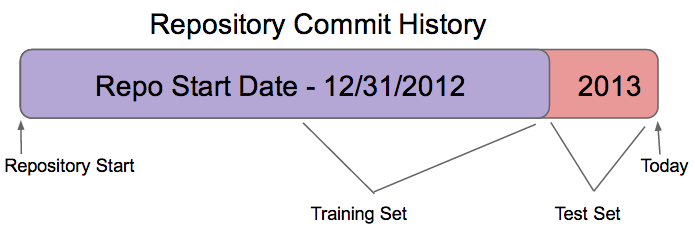
\includegraphics[width=0.75\textwidth]{images/history}
\caption{Testing and Training Sets}
\label{git_comp}

\end{figure}

For training data, we took commits from the final day of 2012 back six months, one year, two years, and to the start of the repository.  The goal here is to see how our results change with more data to train on (and potentially overfit to).  Tables [CITE] and [CITE] show the size and percentage of commits which are buggy respectively.  Notice as time increases, the percentage of buggy commits increases (excepting scala all time).  This seems to be an artifact of our heuristic; older bugs are more likely to have associated bug fixes, and so are more likely to be found by our method.  Without having the actual distribution of buggy commits, we can make no assumptions about its trend over time.        
	
	
	\begin{table}
\begin{center}
    \begin{tabular}{ | c | c | c | c | c |c|}
    \hline
    
Repo & Test Set & 6Mo Train  & 1 Yr Train   & 2 Yr Train & All Train \\ \hline


one &  2304  &  1190 &  2423 & 4367  &  5874 \\ \hline
cyclus & 546  & 389  & 1231  & 1524  & 1616 \\ \hline
git & 2916  & 1369  & 2630  & 5129  & 25869 \\ \hline
jedit & 165  & 301  & 760  & 1401  & 6725 \\ \hline
jquery & 898  & 592  & 925  & 1934  & 4695 \\ \hline
puppet & 2195  & 980  & 2130  & 3854  & 9979 \\ \hline
scala & 1752  & 1347  & 2983  & 5080  & 18644 \\ \hline
scipy & 1873  & 546  & 1130  & 1786  & 8162 \\ \hline


 
\end{tabular}
\end{center}\caption{Size of Training and Test Sets}
\label{tab:size}
\end{table}

	\begin{table}[h]
\begin{center}
    \begin{tabular}{ | c | c | c | c | c |c|}
    \hline
    
Repo & Test Set & 6Mo Train  & 1 Yr Train   & 2 Yr Train & All Train \\ \hline


one  & 23.1 & 26.4 & 30.2 & 35.4 & 37.7 \\ \hline 
cyclus  & 30.6 & 44.4 & 50.6 & 54.9 & 55.9 \\ \hline 
git  & 13.9 & 22.1 & 22.5 & 23.4 & 39.7 \\ \hline
jedit  & 6.7 & 13.9 & 24.7 & 23.1 & 47.3 \\ \hline
jquery  & 35.7 & 43.2 & 46.6 & 53.9 & 58.6 \\ \hline 
puppet  & 18.7 & 20.0 & 26.1 & 29.1 & 44.1 \\ \hline 
scala  & 27.2 & 45.3 & 48.8 & 50.3 & 48.9 \\ \hline 
scipy  & 18.8 & 23.6 & 23.6 & 24.7 & 35.5 \\ \hline
\end{tabular}
\end{center}\caption{Bugginess of Training and Test Sets}
\label{tab:buggy}
\end{table}

%\begin{figure}
  %  \centerline{
%        \subfigure[Git]{%
%            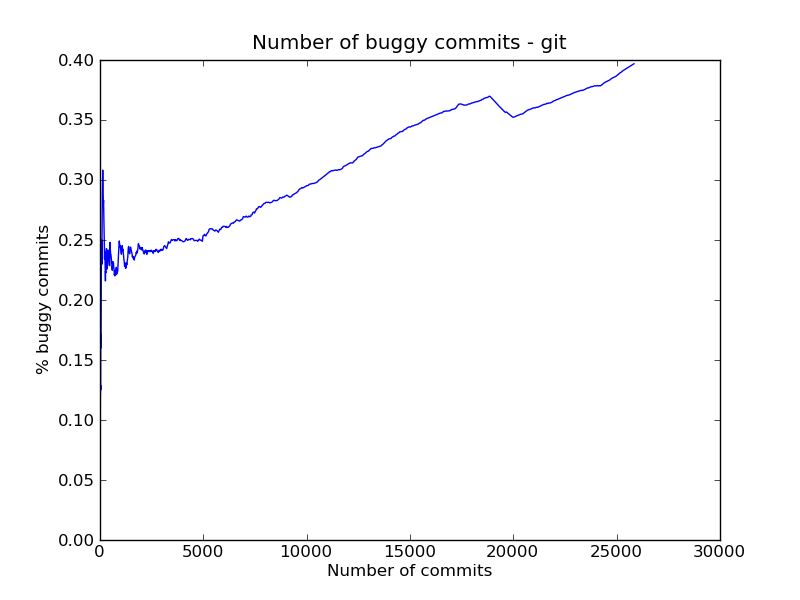
\includegraphics[width=0.4\textwidth,height=.3\textwidth]{images/perc_buggy_git}
%        }%
   %     \subfigure[Puppet]{%
      %     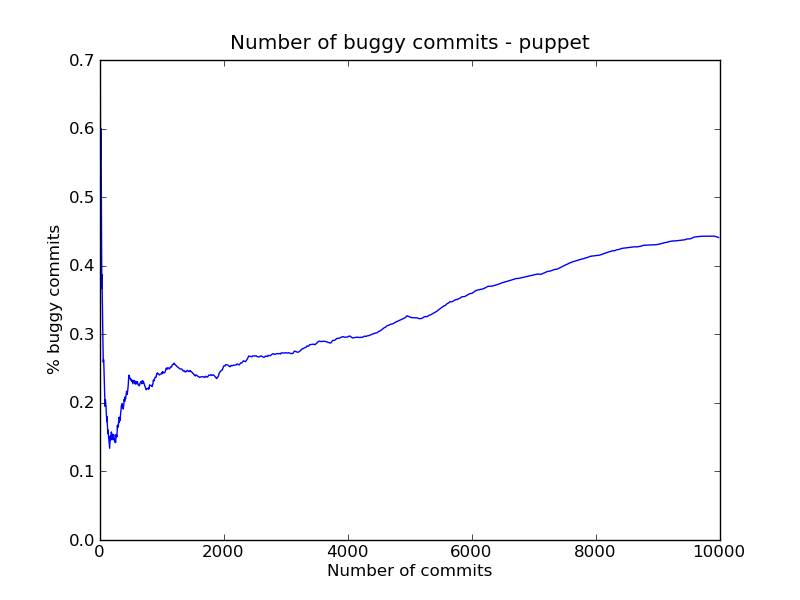
\includegraphics[width=0.4\textwidth,height=.3\textwidth]{images/perc_buggy_puppet}
   %     }
   %     \subfigure[Scala]{%
   %         \includegraphics[width=0.4\textwidth,height=.3\textwidth]{}
      %  }%
 %}
% \caption{Percent Buggy Commits over Time}
%\end{figure}

\begin{figure}[H]%
\centering
\subfloat[Git]{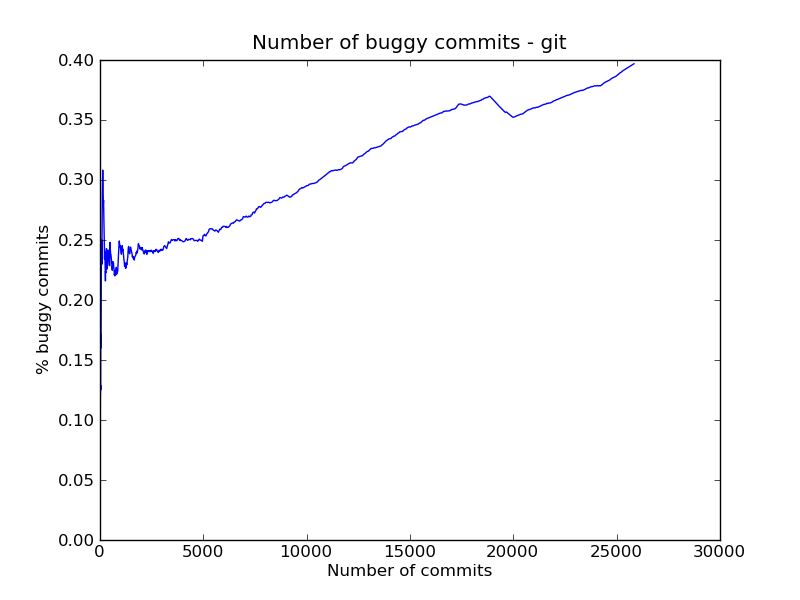
\includegraphics[width=0.5\textwidth]{images/perc_buggy_git}}\hfill%
\subfloat[Puppet]{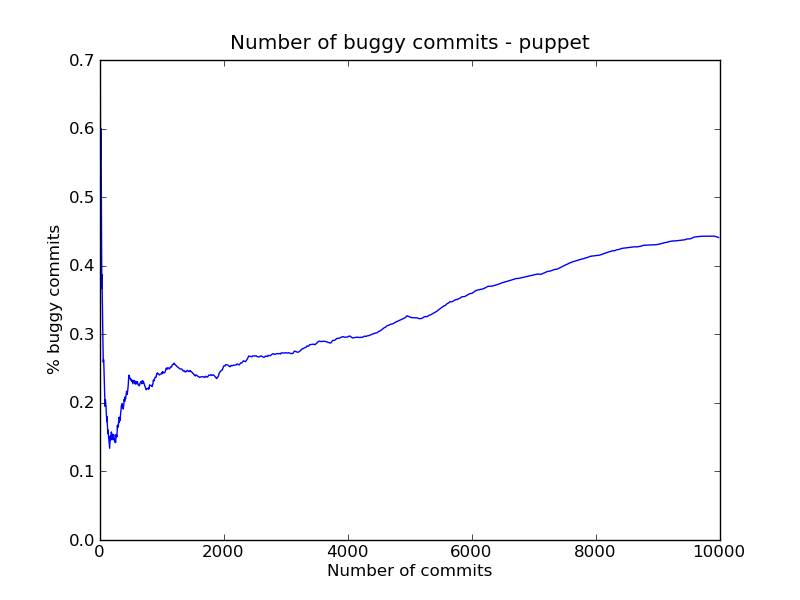
\includegraphics[width=0.5\textwidth]{images/perc_buggy_puppet}}
\caption{Percent Buggy Commits over Time}
\end{figure}


To compare our features against some baseline, we created a �random weighted coin� classifier which calculated the percent buggy in a training set, and used this percentage as the weight on a random buggy/clean coin for each test instance.  We feel this represents a better floor against which to compare our results than simply using a fair coin.  To compare the effectiveness of attribute and message features, we also trained classifiers using only attribute features, only message features, and both sets of features.  


\subsection{Classifier Accuracy}

 \begin{figure}
\centering
	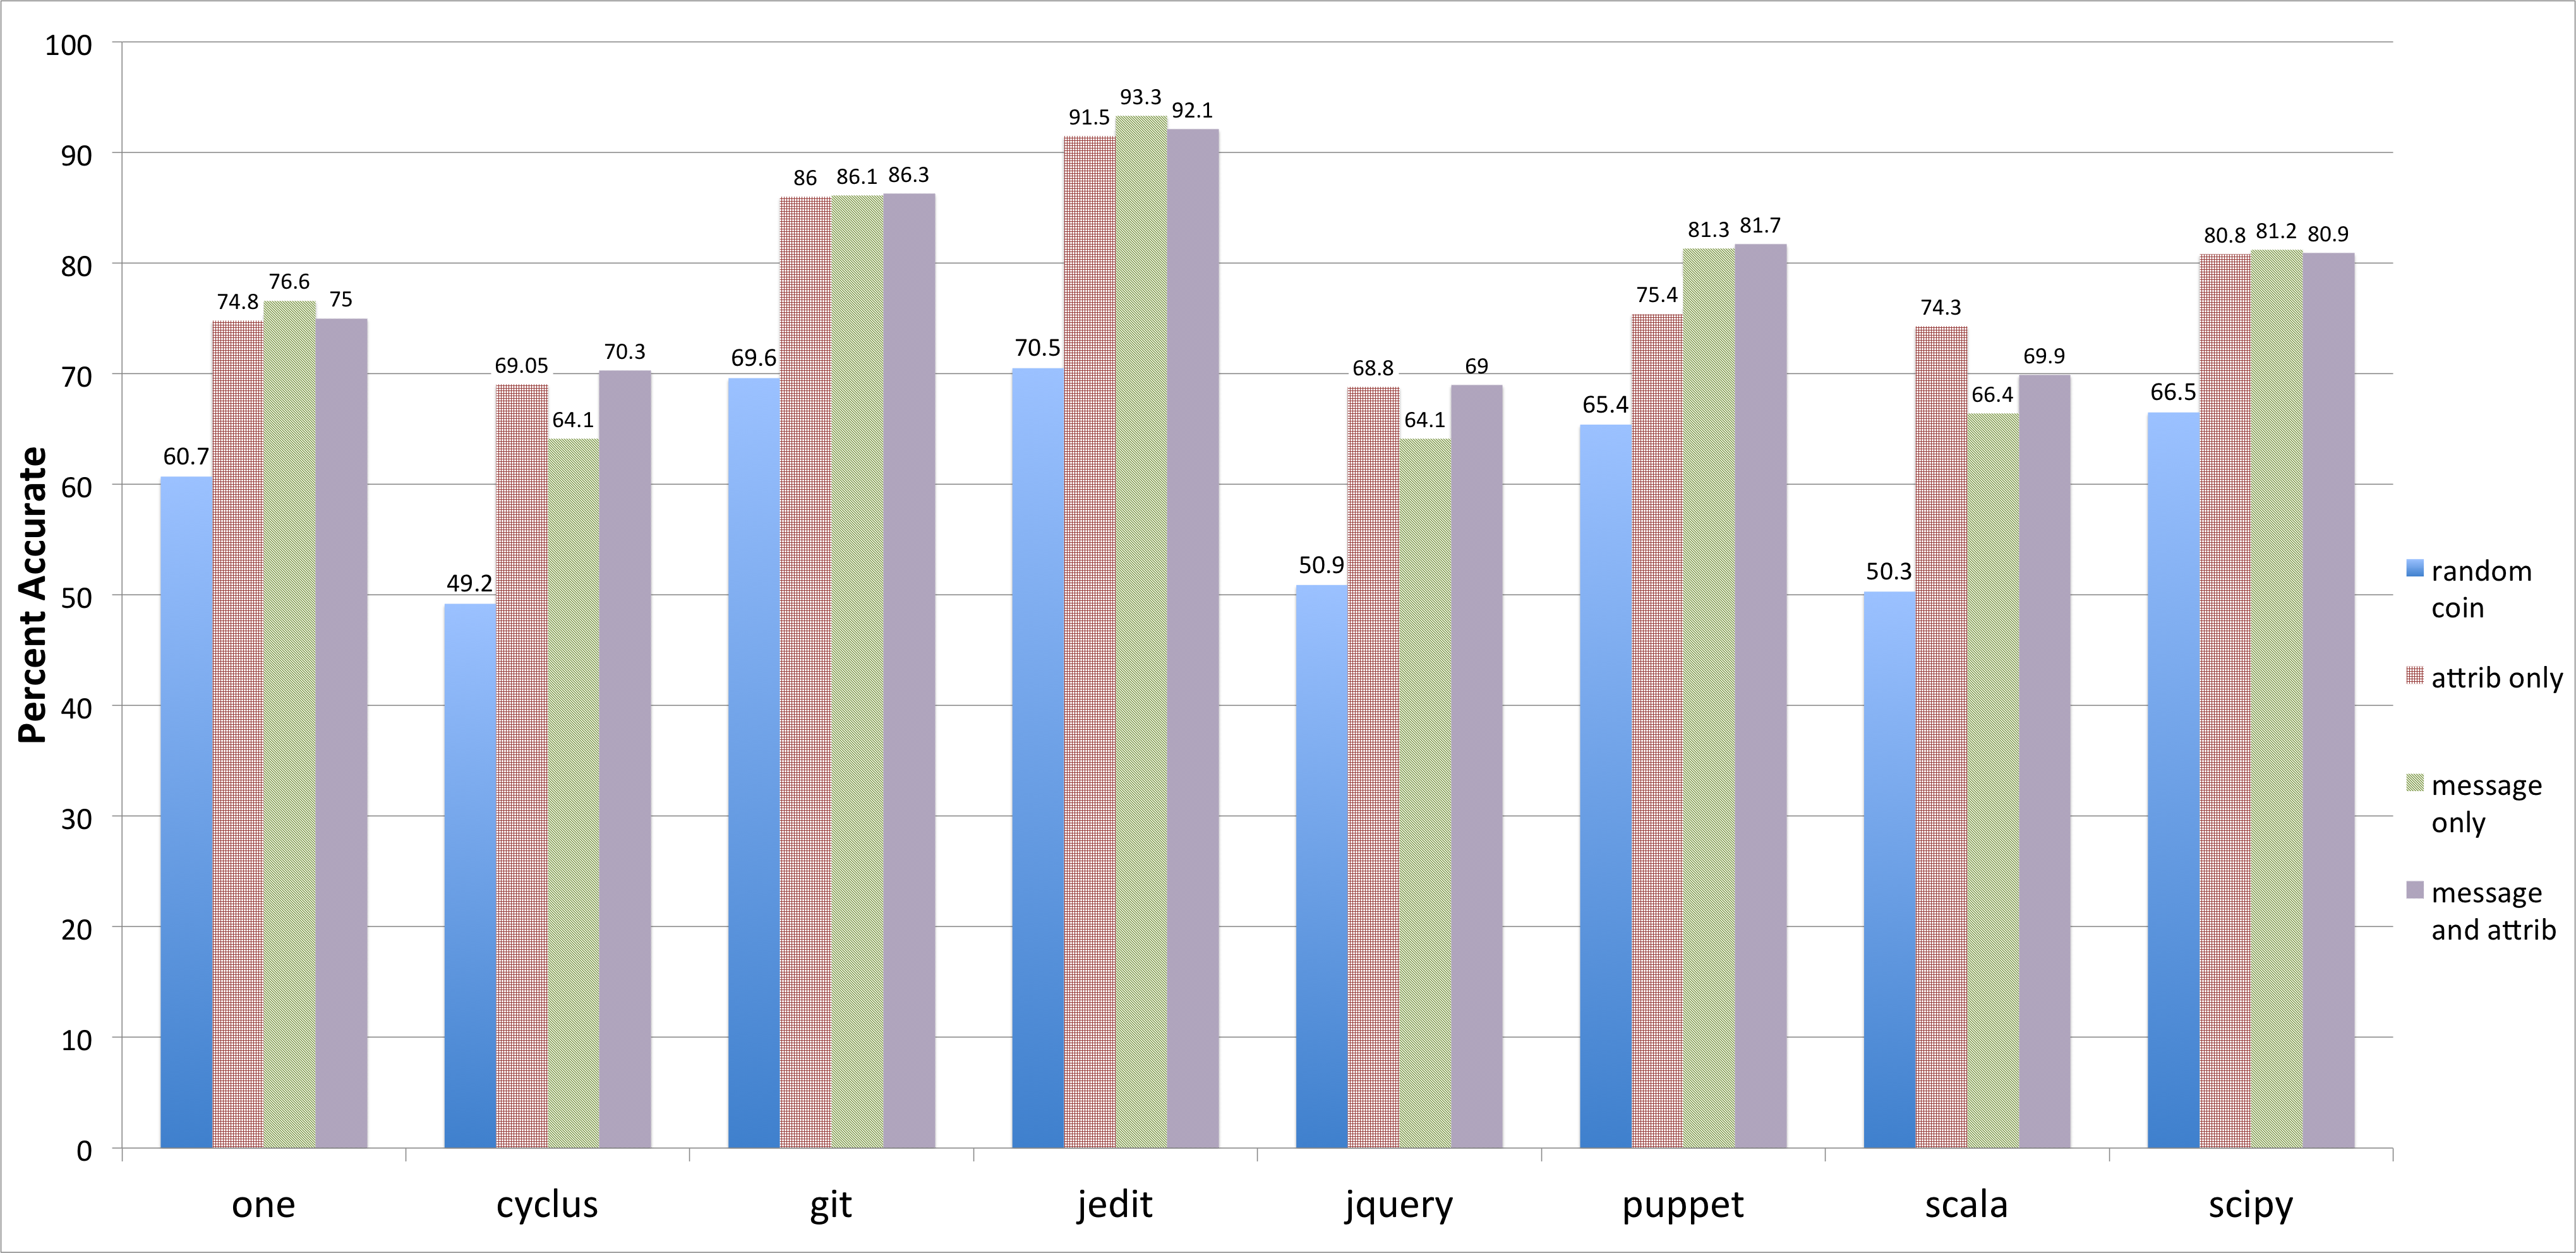
\includegraphics[width=1.0\textwidth,height=.5\textwidth]{images/learner_comp}
\caption{Comparison of Feature Results - 1 Year}
\label{git_comp}

\end{figure}
Figure [CITE] contains our accuracy results using one year of training data.  Results for random coin vary but in general are about fifteen to twenty points lower than the rest of the classifiers.  Using attribute features only tends to work as well or slightly better than message features, with big drops only occurring in cyclus and jquery.  Using both sets of features is comparable to only using one, though it appears more similar to message attributes.
 
As much as we would like it to be otherwise, the 93.3 \% accuracy seen by jedit is more than a little misleading; the jquery test set is only 6.7\% buggy, and so the jedit classifiers simply guess clean for every instance. This is true for the majority of message-only feature classifiers; only cyclus and jquery classifiers ever classify any test commits as buggy.  The results from these classifiers are still promisingly higher than our baseline, which leads us to believe that our features do have some non-random correlation with clean and buggy commits.   All of our attribute-trained and attribute/message-trained classifiers have non-trivial decision boundaries.  To get a better idea of how well our classifiers actually are at correctly predicting commits as buggy, we examine precision/recall graphs for cyclus, scala (the two repositories with non-trivial decision boundaries) and scipy by varying the ensemble classifier threshold from 0.0\% agreement (always classify buggy) to 100\% agreement.  

\begin{figure}[H]%
\centering
\subfloat[Cyclus]{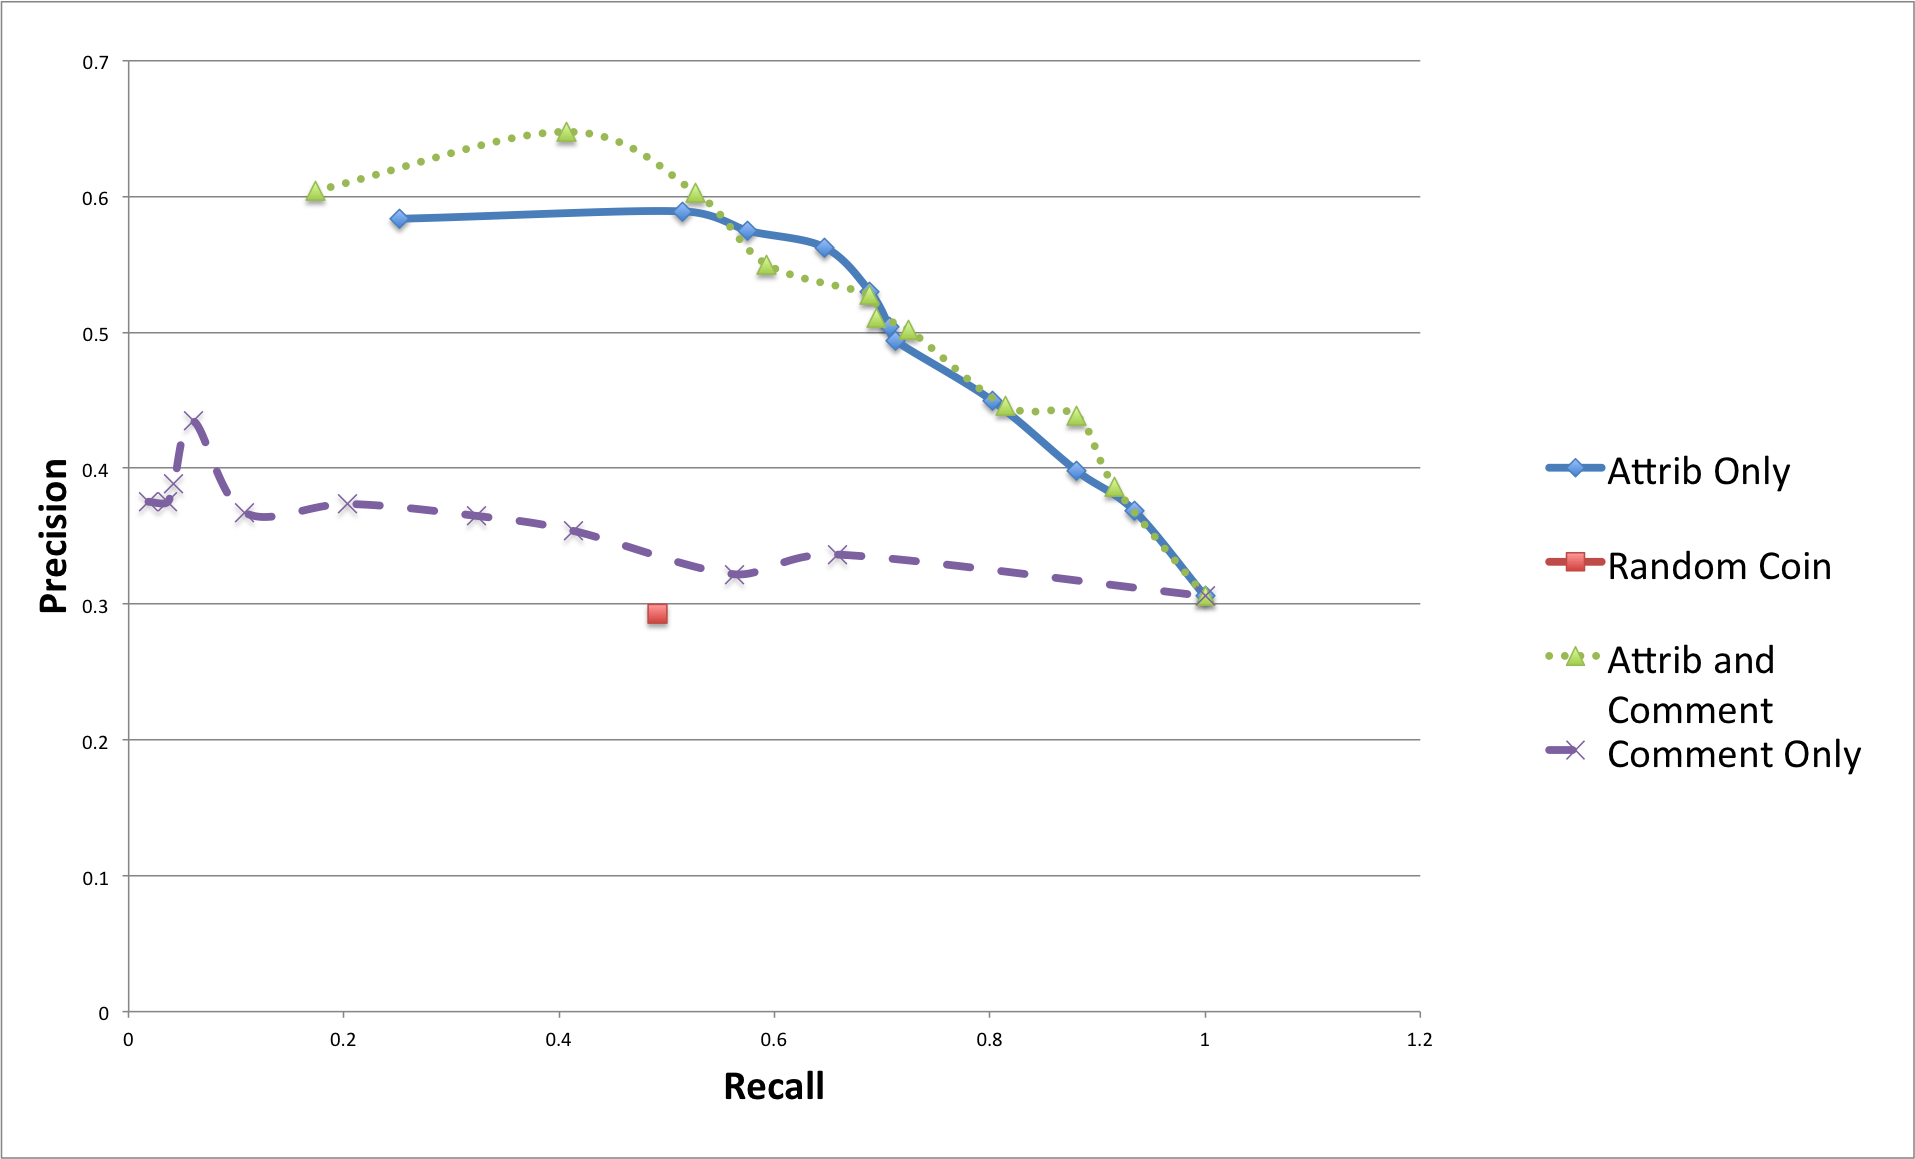
\includegraphics[width=0.5\textwidth]{images/cyclus_pr}}\hfill%
\subfloat[Scala]{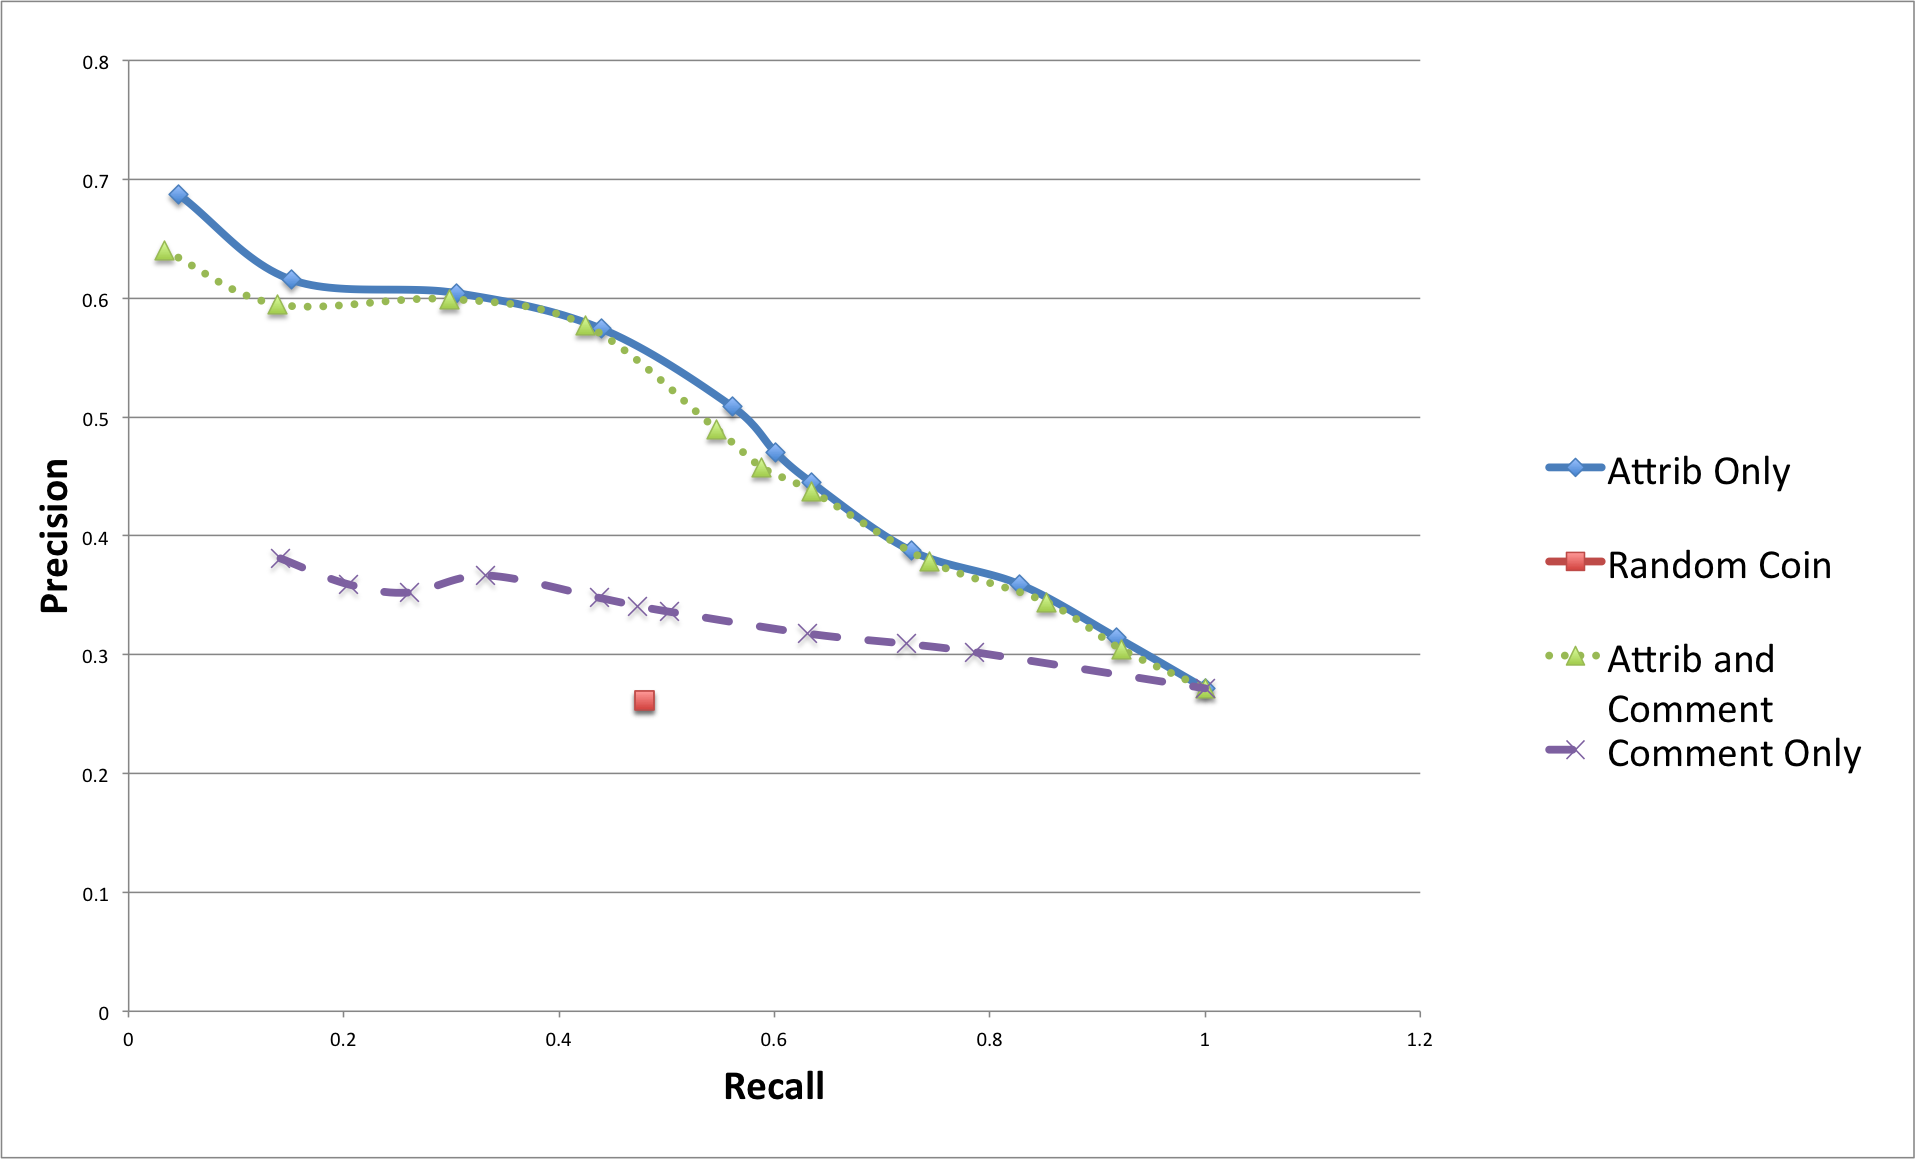
\includegraphics[width=0.5\textwidth]{images/scala_pr}}\\
\subfloat[Scipy]{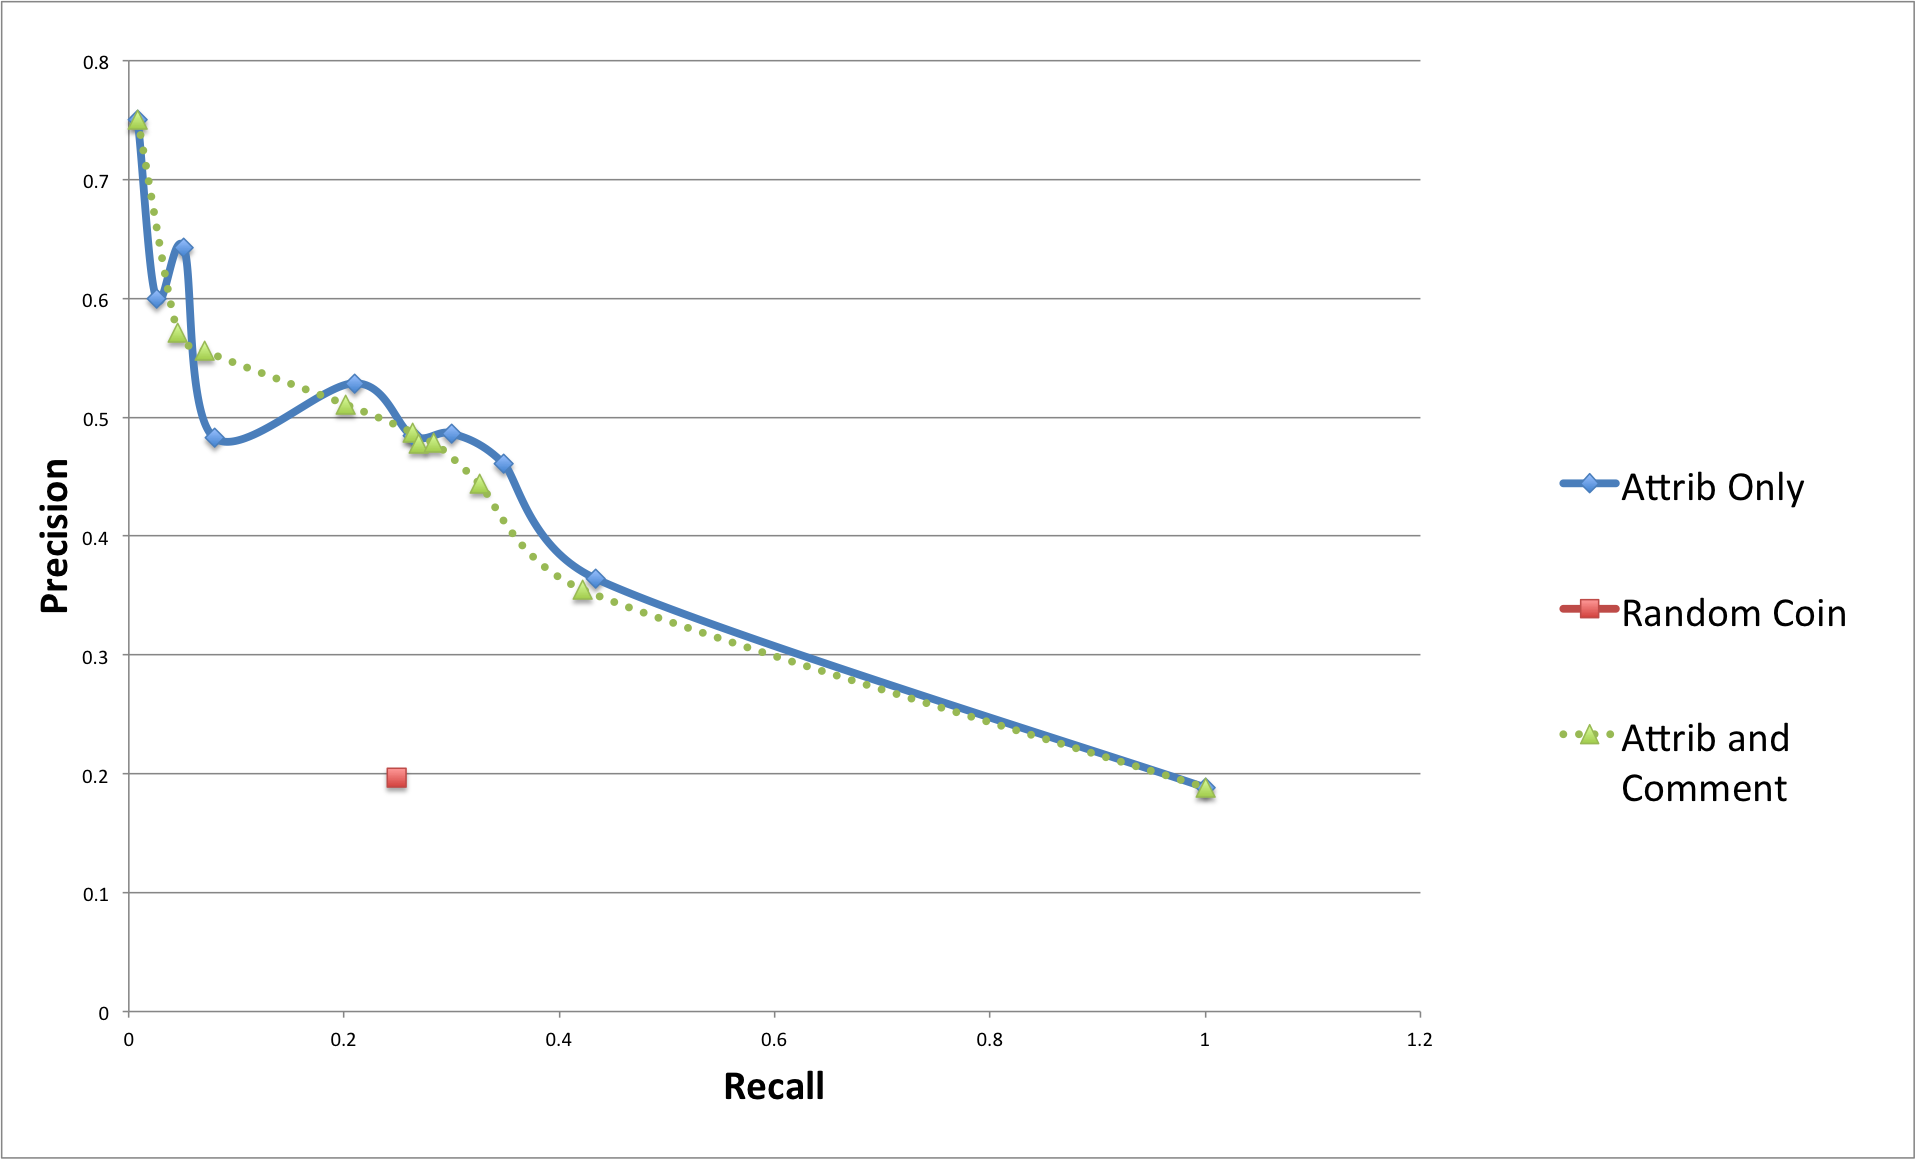
\includegraphics[width=0.5\textwidth]{images/scipy_pr}}\hfill
\subfloat[Cyclus - ROC graph]{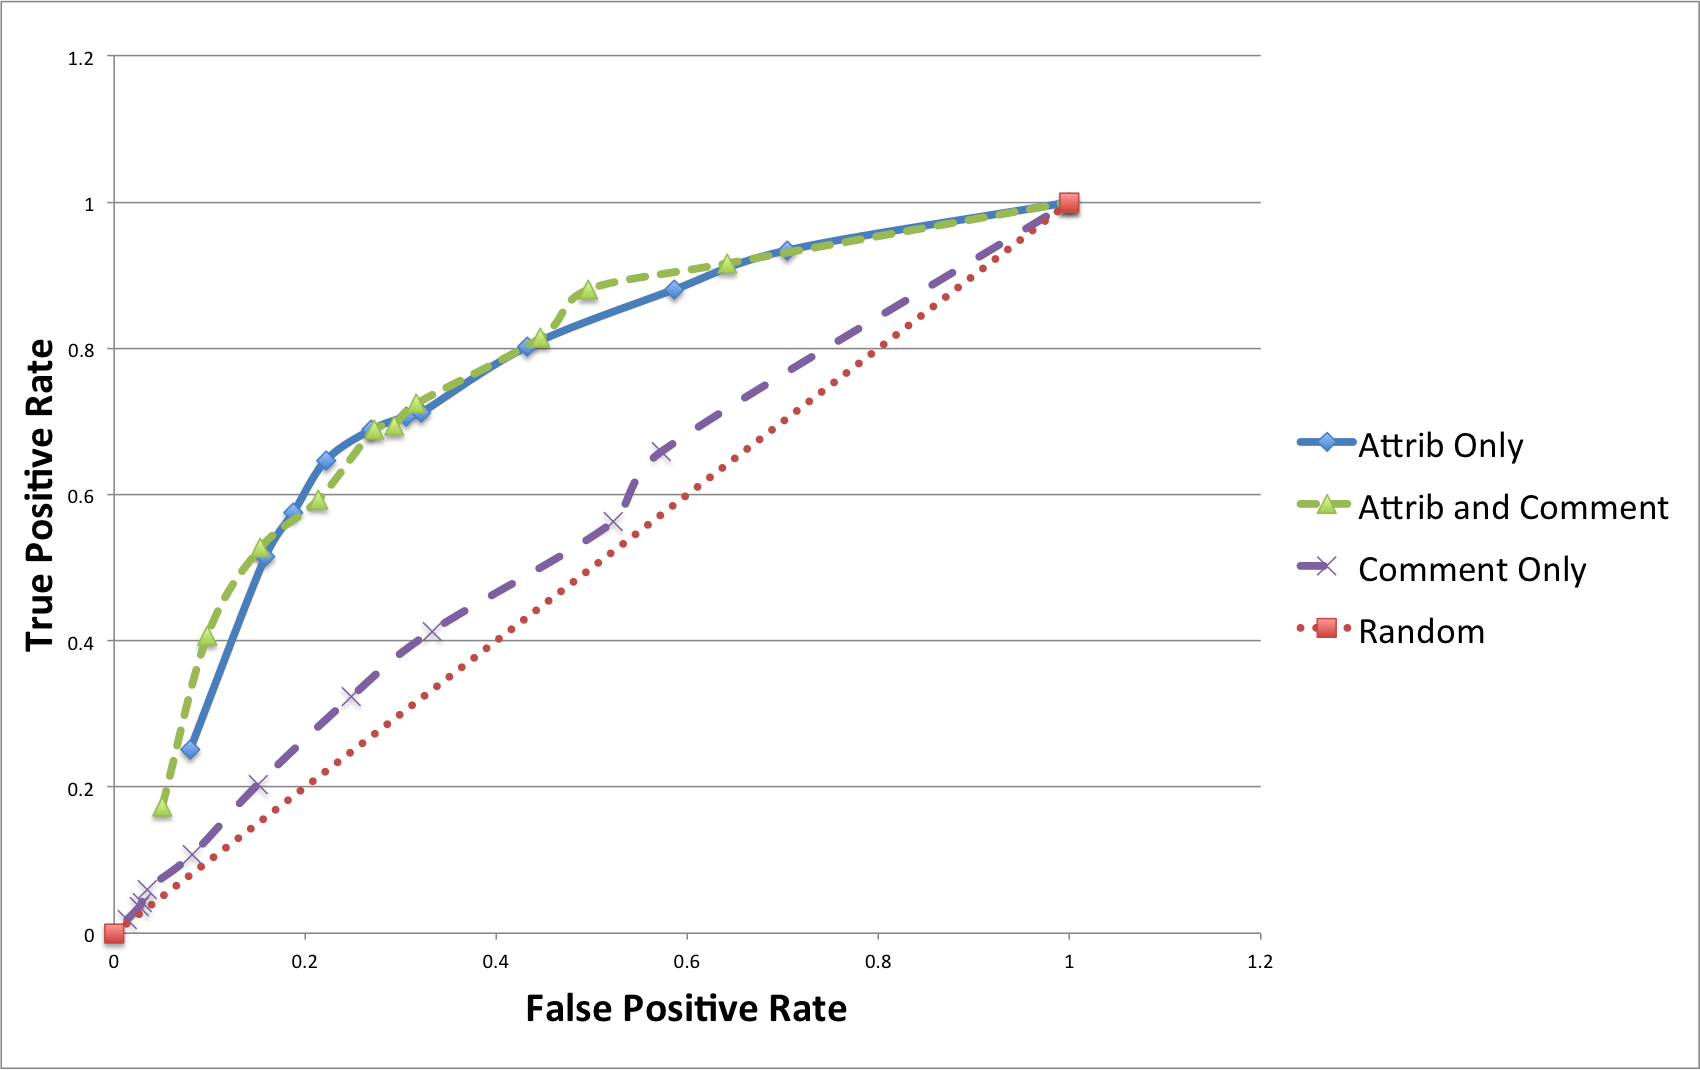
\includegraphics[width=0.5\textwidth]{images/cyclus_roc}}\hfill

\caption{Precision Recall Graphs}
\end{figure}

As these figures show, using only comments is better than random.  At the same time, using just comments performs worse in all cases than using attribute data.  Using attribute data performs about as well as training on both attribute and comment features.  This leads us to several conclusions.  First, both sets of attribute and comment features are more predictive than random.  Comparatively, attibute features are a much better approximation of a commit than comment features.  Combining attribute and comment features provide  little additional performance benefit over simply using attributes.     


\subsection{Training Set Variation}

 \begin{figure}[h]
\centering
	\subfloat[Accuracy]{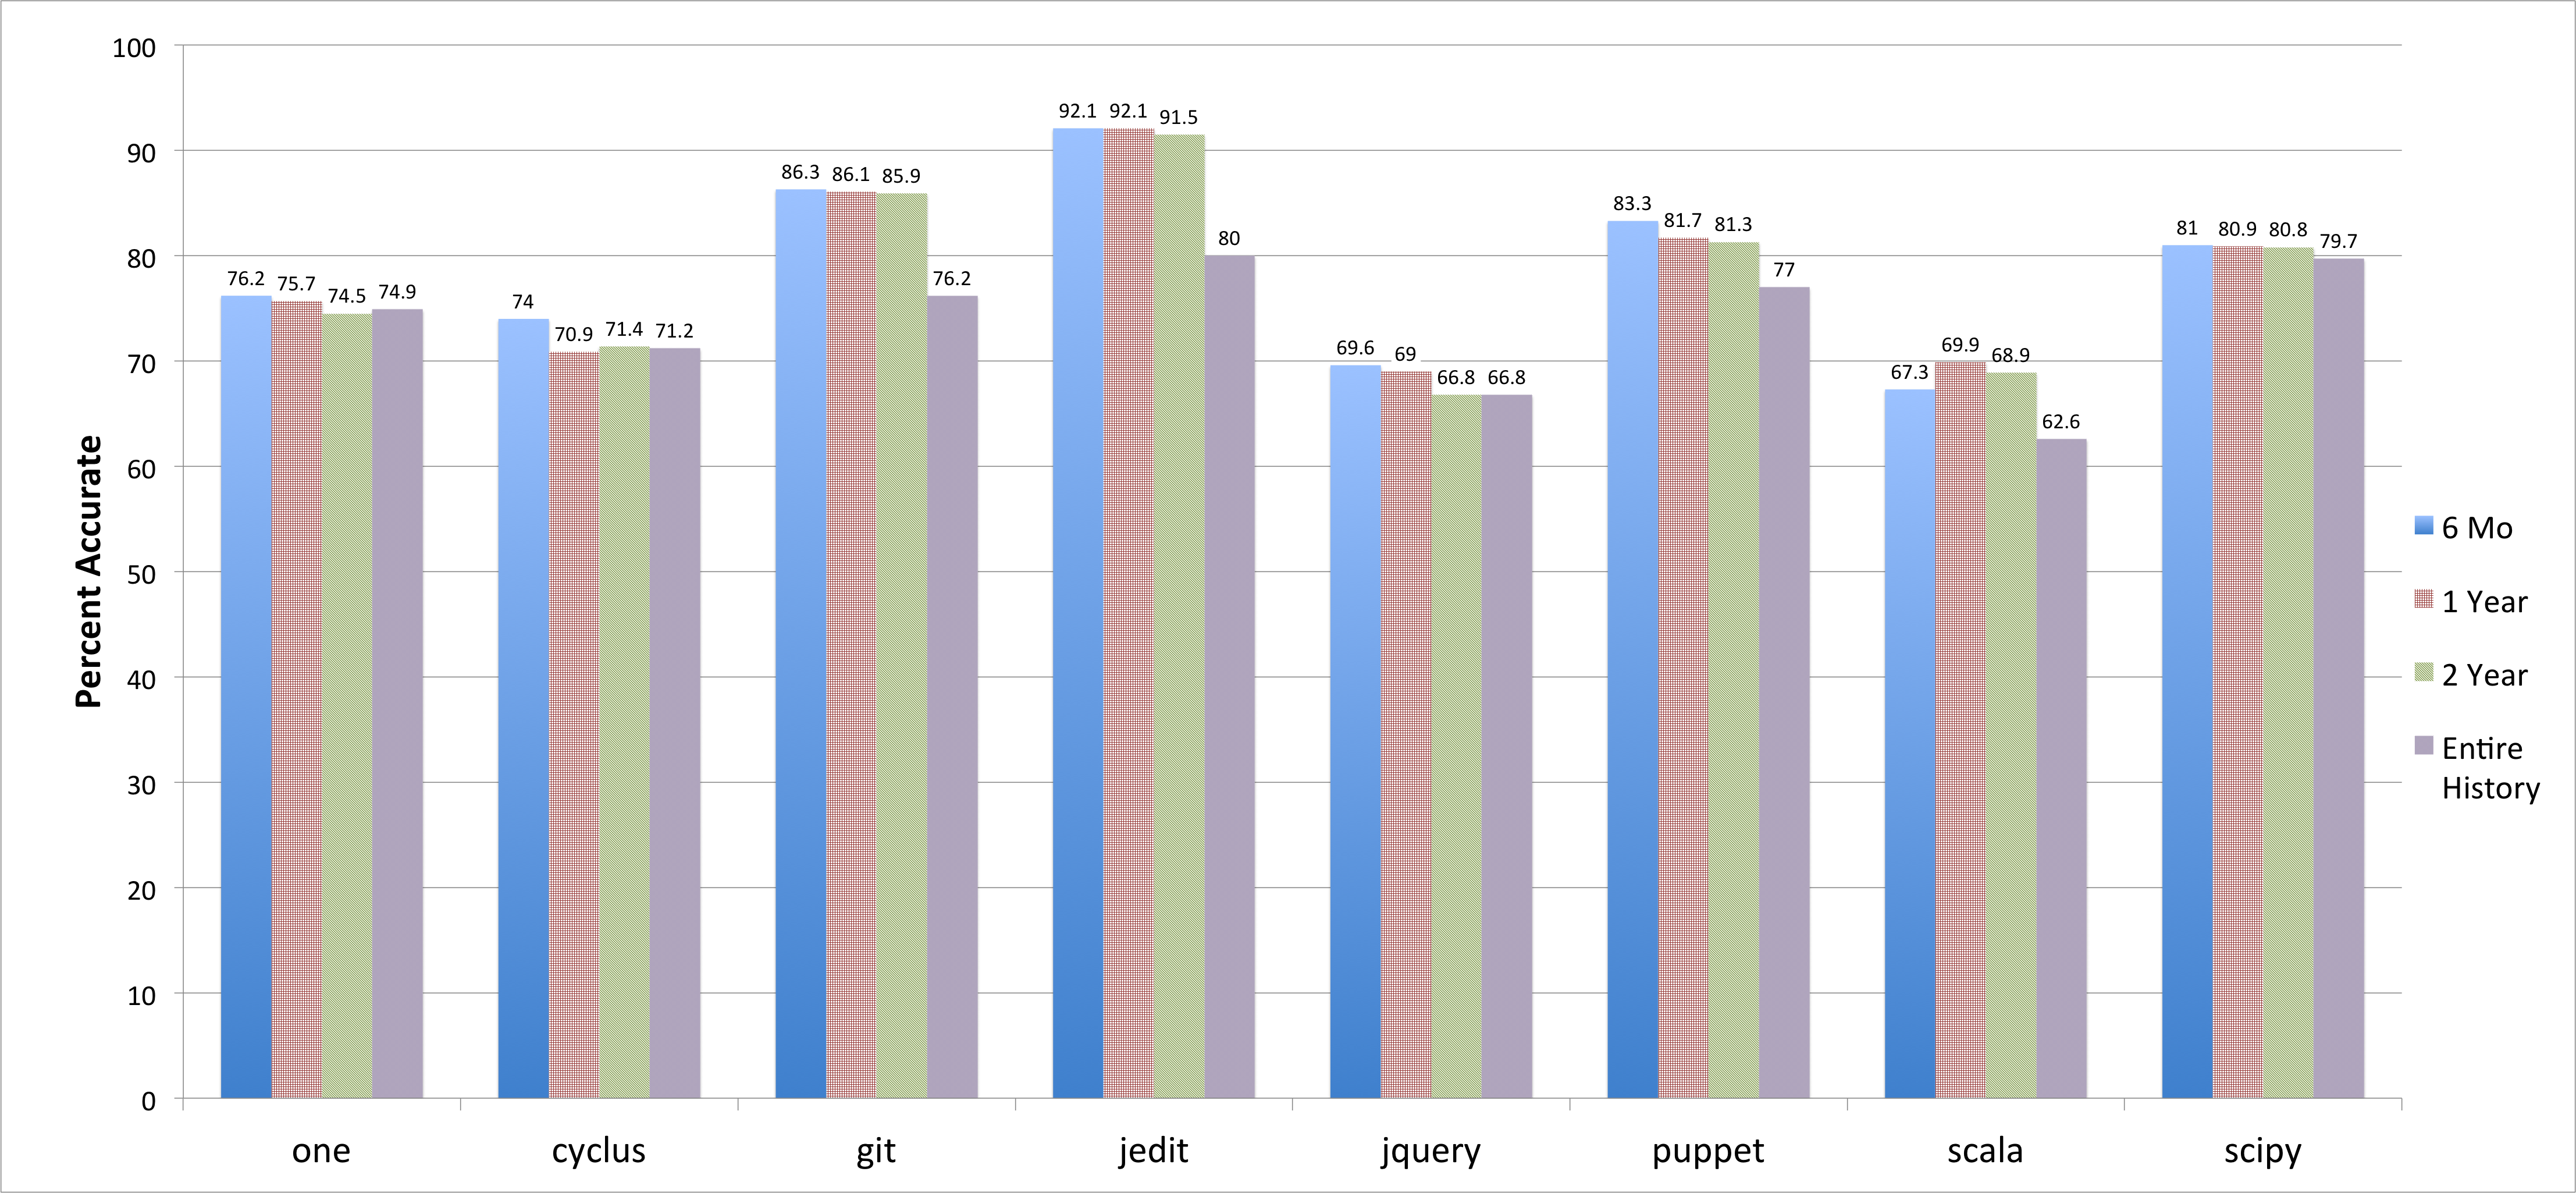
\includegraphics[width=0.5\textwidth,height=0.3\textwidth]{images/time_comp}}\hfill
	\subfloat[Precision Recall Graph]{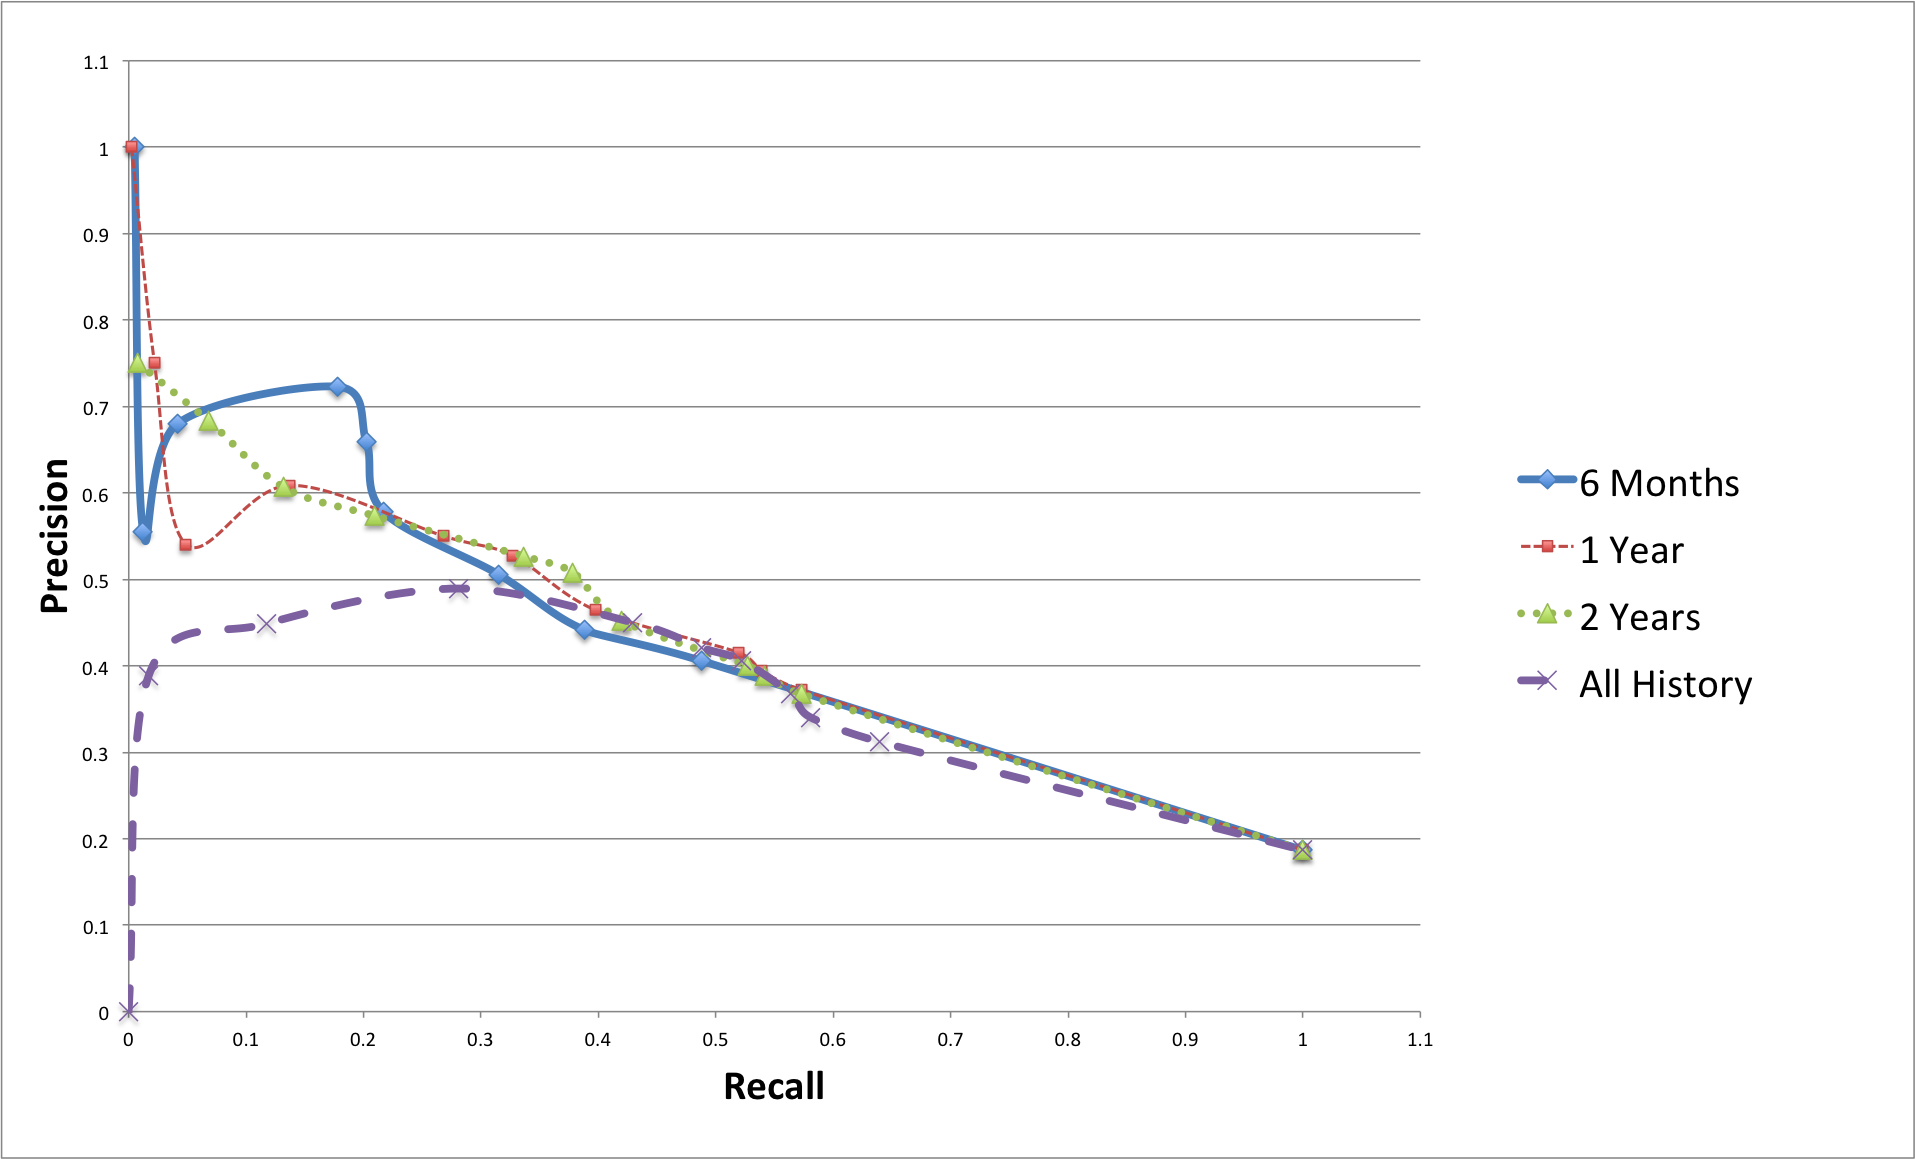
\includegraphics[width=0.5\textwidth]{images/time_pr}}\hfill
	
\caption{Training Data Size - Message and Attributes}
\label{git_comp}

\end{figure}
Accuracy across repositories tended to trend downward as the time frame from the training set increased.  Not visible in table [CITE] is the fact that for six months data sets, the likelihood  of trivial decision boundaries seems to increase.  On the other end of the spectrum, however,  it seems clear that using all of the data introduces too much noise.  Some of these projects predate git and almost certainly were originally in another version system.  Overall, it seems likely to us that recent commits are more representative of commits in the near future, which would explain the drop in results.  From our work, we suspect one to two years is the �optimal� range of sizes, though this will obviously be different for each repository, depending on how often they make commits.  We did not test this, but it might also be beneficial to allow a period of time between the training data and the most recent commit; this space could help reduce false negatives by allowing a reasonable amount of time for bug fixes for the training data to be added. 



\subsection{Cross Repository Training}

A year of repository data before being able to use a tool seems like a fairly high price of admission.  Being able to substitute another repository�s history for your own with little to no hit in accuracy seems like it would make our tool more applicable.  Furthermore, what does this say about commits if commits from two unrelated repositories are similar enough that one can be used to train the other?  To answer these questions, we decided to use git�s commit history to train our classifier and test on the other seven repositories.  Scipy and git were chosen because they were large repositories with good performance and non trivial decision boundaries.  In order for training and testing data to be compatible, the user feature had to be removed from all data sets. 

 \begin{figure}[h]
\centering
	\subfloat[Accuracy]{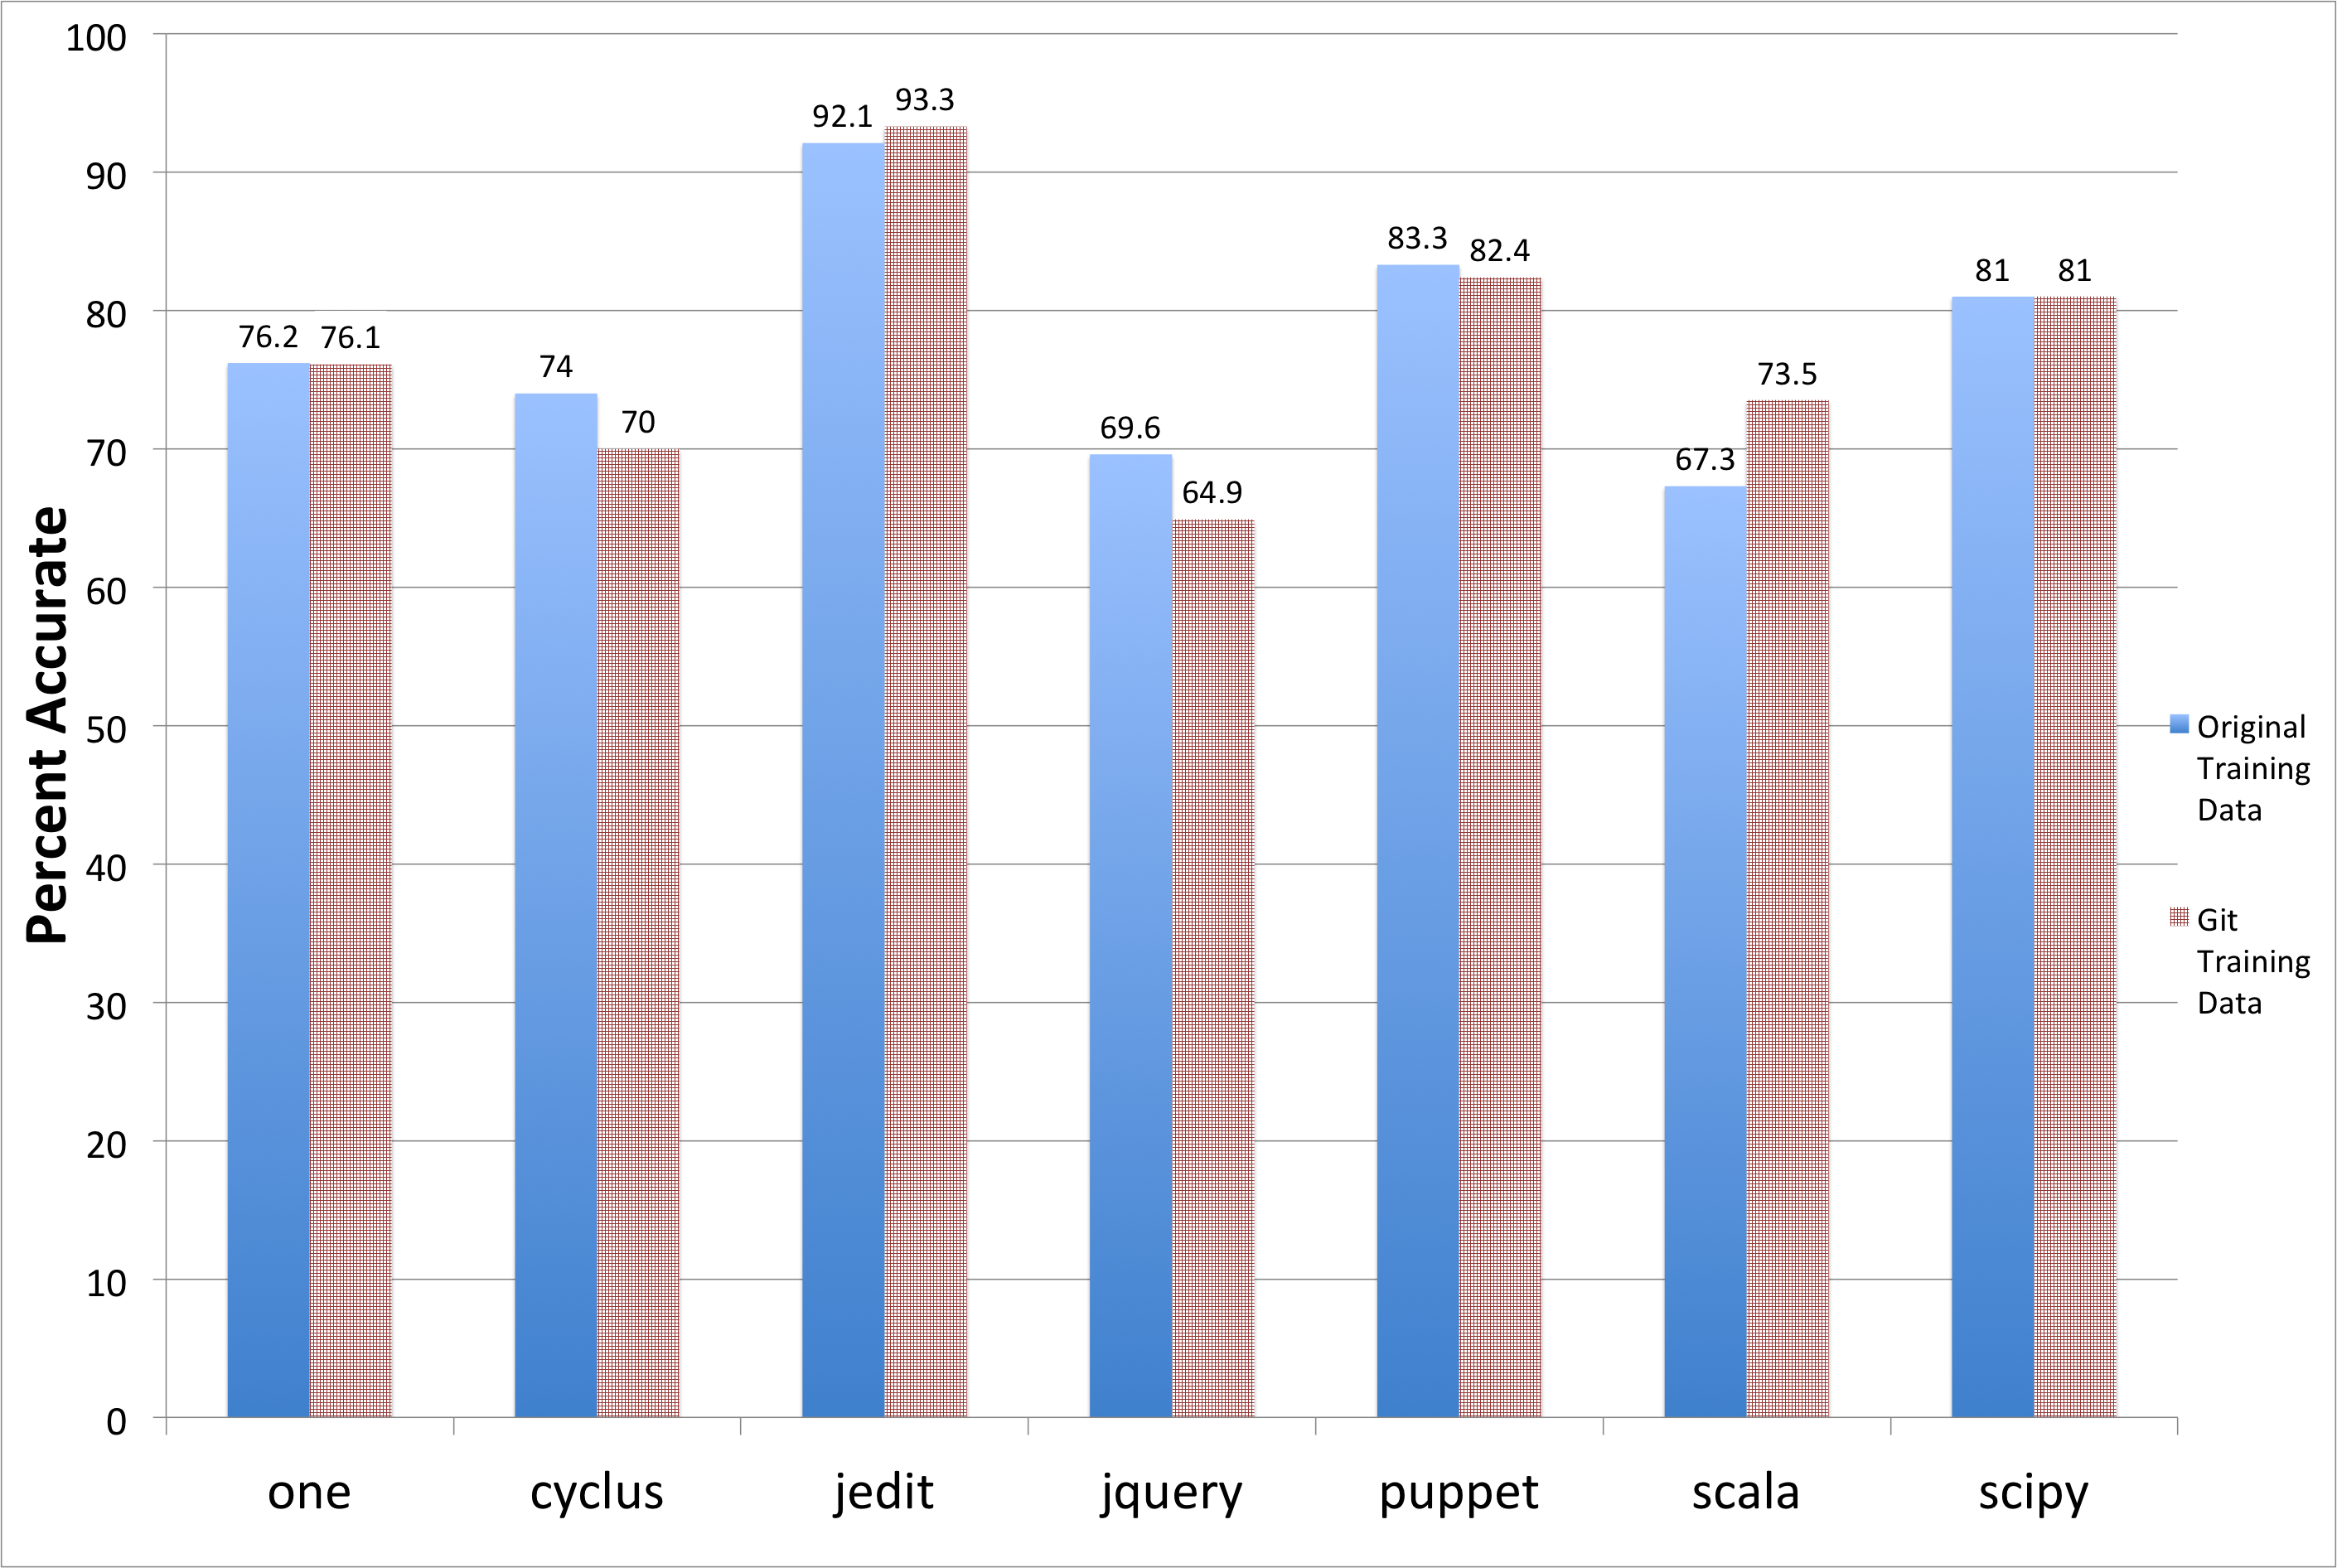
\includegraphics[width=0.5\textwidth,height=0.3\textwidth]{images/git_comp}}
	\subfloat[Precision Recall]{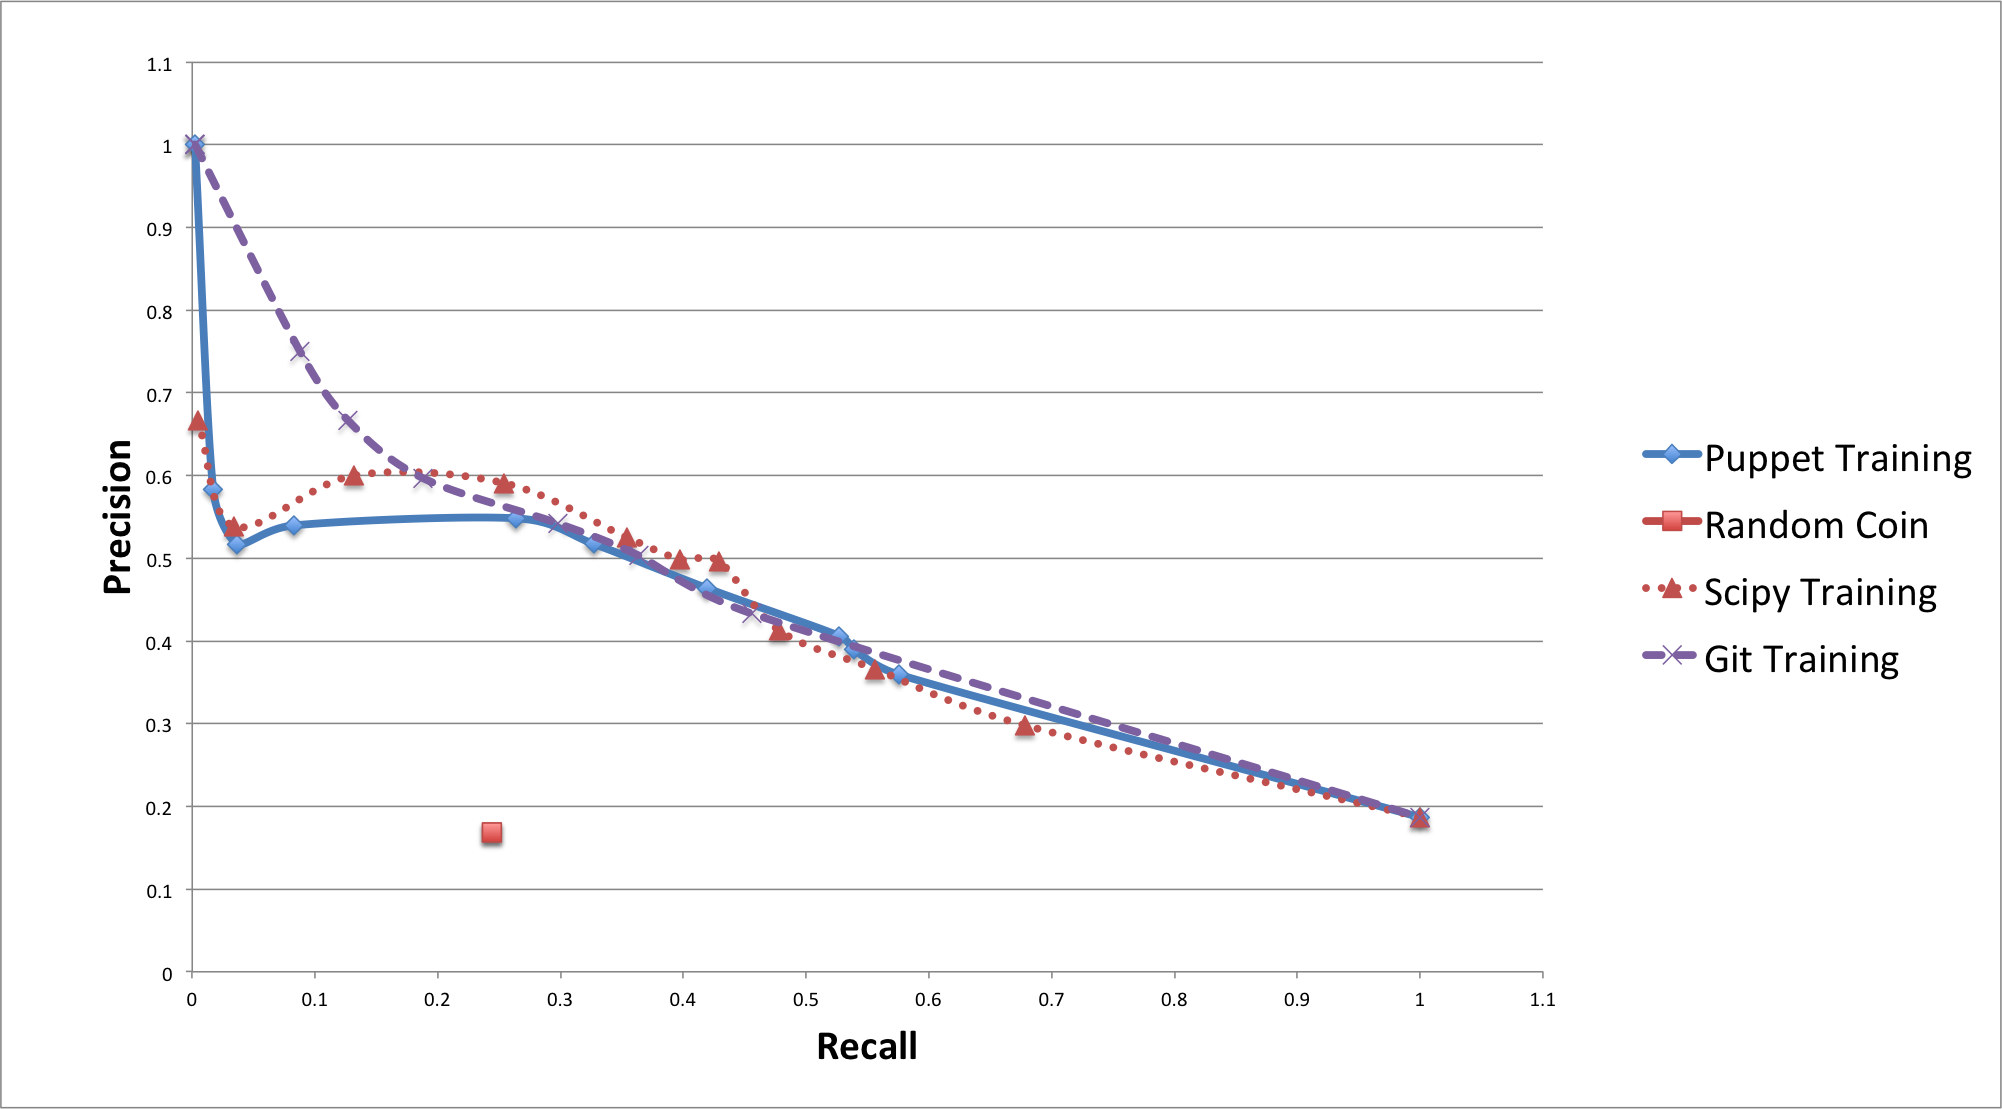
\includegraphics[width=.5\textwidth]{images/git_pr}}
\caption{Training With Git and Scipy - 1 Months, Message and Attribute Data}
\label{git_comp}

\end{figure}

In general, results tended to be comparable to those using their respective data sets.  The cross-repository classifier accuracies displayed the same trend of slow decrease as training data size increased, with a noticeable drop when all training data was used.  

This comparable performance indicates to us that using a classifier trained on another repository is a valid proxy for repositories that do not have their own history.  It also seems that the distribution of message and commit attribute features we use do not vary much across repositories.  More work would need to be done to give such a claim actual weight, but if our features have global, general boundaries, could we use this information in some kind of prescriptive fashion, a la �keep your commits to X lines added if possible�. Or would knowledge and enforcement of this information simply shift the boundary?   

\section{Threats to Validity}

There are several potential threats to the validity of our results.  The heuristic used in classifying past commits represents a multifaceted threat.  First, though [CITE] has presented some evidence that this method works well in practice, there is no evidence to support that these results generalize well.  As we mined neither of the two projects they studied, it is possible that our approximation of the true distribution of clean and buggy commits is flawed.  Even if we had mined those repositories, it is possible in the eight years between the writing of [CITE] and now that the heuristic does as well.  Another potential problem this heuristic introduces is that our ensemble learner is attempting to learn this approximation.  If the approximation does not closely match the actual distribution, then the results we present are in no way an indication of how our tool would perform against actual commits.

Another potential threat is the repositories we chose.  While we attempted to pick a representative sample of the open source projects in development, this excludes closed source projects. Also, we only mined english-speaking repositories, which is required by our heuristic classification and all of our message features.  We made no attempt to take into account differences and eccentricities of the individual repositories we did mine.  It is possible (even likely) that these eccentricities are to account for the variation between repositories.   

\section{Future Work}
There are many potential avenues of future work that could stem from this work. One of the most important aspects of a commit that has purposefully been ignored in this work is the committed code itself.  It is possible to investigate lightweight analysis of code changes could provide valuable indications of bugginess without making training our classifier intractable.  Also, we believe looking at commit messages through the lense of more advanced natural language processing techniques could yield additional benefits.

Our results have shown commits are not especially repository specific, but we believe they could potentially be user-specific?  Does it make more sense to have a user-specific classifier that examines the user�s commit history across the repositories they have contributed to than to have a single classifier that predicts labels for potentially many users. Studying this would not require much additional new work to be done beyond mining new repositories and organizing training sets.  If user-specifc commits are in fact better predictors of bugginess, additional work would need to be done to ensure user�s do not cherry-pick their training data to give an overly positive but invalid bias.       

Another potential way to approach this problem is through semi-supervised learning.  Rather than attempting to classify all commits as clean or buggy which  requires automatic heuristics, the classifier could simply keep the distribution of commit features stored, some subset of which the user has manually classified as clean and buggy.  The model could then be set up to request labels on past commits that it finds interesting or questionable.  

\section{Concluding Remarks}

% references section

\addcontentsline{toc}{section}{Bibliography}
\begin{thebibliography}{99}
\end{thebibliography}



% that`s all folks
\end{document}




